\documentclass[10pt,twocolumn]{article}
\usepackage[letterpaper,margin=0.5in]{geometry}
\usepackage{graphicx}
\usepackage{caption}
\usepackage{booktabs}
\usepackage{tabularx}
\usepackage{array}
\usepackage{float}
\usepackage{url}
\usepackage{pdflscape}
\usepackage{enumitem}
\setlength{\columnsep}{0.24in}
\setlength{\parindent}{0pt}
\setlength{\parskip}{3pt}
\setlength{\textfloatsep}{5pt}
\setlength{\intextsep}{4pt}
\captionsetup{font=footnotesize,skip=2pt}
\setlist{nosep,leftmargin=*}
\newcommand{\p}[1]{\path{#1}}
\newcommand{\tightcaption}[1]{\captionof{figure}{#1}}

\title{Scientific Progress Assessment: Independent Axial Seamount Reproduction}
\author{Axial Modeling Project}
\date{22 October 2026}

\begin{document}
\maketitle
\vspace{-1.1em}
\begin{center}\small
Repository: \p{github.com/mhemmett/axial-modeling} \quad
HEAD: \texttt{e7d9dcc} \quad
Branch: \texttt{feat/independent-paper-figure-results}
\end{center}
\vspace{-0.7em}

\textbf{Decision.} The project has a working, bounded PyLith workflow, independent BPR processing, steady thermal-property transfer, and useful verification tools. Those are credible software and data-handling accomplishments; they do not yet recover a defensible pressure threshold or eruption time. The principal obstacle is unstable reservoir compliance on nonnested, coarse meshes, compounded by unmeasured rheology and failure properties and an incompletely validated basal boundary. I recommend pausing broad model development and funding at most one gated mesh-convergence study. Past expenditure is not a scientific reason to continue.

\section*{What is implemented}
The code solves elastic and generalized Maxwell deformation around a pressurized ellipsoidal cavity, solves steady conduction, maps temperature to cellwise modulus and viscosity, and postprocesses tensile and Mohr--Coulomb indicators and connected paths. A hydrothermal case raises conductivity in the shallow crust. This is one-way thermal-to-mechanical coupling: mechanics does not feed heat back, and no fluid-flow or permeability equation is solved. Failure is a stress-based proxy, not a plastic fault-slip calculation.

The 50 by 50 by 10 km box and 6 by 3 by 1 km reservoir follow project direction and the written source geometry; the reservoir is rotated to N30$^\circ$W. The project uses a fixed base in its main calibrations although the paper specifies a Winkler foundation. A separate gravity and lithostatic reference-state diagnostic now iterates a regional finite spring. Its density profile is depth-averaged and approximate, its solver accepts an initial equilibrium residual of $5.4\times10^3$ under a $10^4$ absolute tolerance, and its station response changes markedly on the coarse mesh.

\textbf{Recovery of scientific findings is limited.} The four rheology paths and expected temperature-dependent property contrasts run, but branch viscosities and fractions are synthetic, the printed modulus equation conflicts with its stated limits, and the project substitutes a directed 50-to-20 GPa law. Thus the property maps are qualitative implementation evidence, not quantitative agreement. Event pressure histories are inversions of BPR displacement, not measured magma pressures. Neither recurrence nor independent eruption timing is predicted. The source's main inference about reservoir overpressure and through-going failure is unresolved: repository screens have produced both failure at low pressure and no joint failure in the updated lithostatic check, depending on assumptions. This is not a robust contradiction or confirmation.

\section*{Evidence and validation}
Four-case raw-channel fits use 309 daily Center/South pairs for 1998 and 314 for 2011. Current local summaries give Center RMSEs of 0.093 and 0.124 m, but held-out South RMSEs of 0.523--0.541 and 0.667--0.687 m. The 2011 South observations deflate by about 1.5 m while modeled changes are about 0.4 m. Fitted pressure changes span approximately $-110$ to $+13$ MPa in 1998 and $-84$ to $+4$ MPa in 2011; these are inversion outputs, not independent pressure measurements. Center fits include eruption deflation and later records, so they cannot predict eruption timing. Tide, ocean variability, and drift remain in raw channels. Corrected-channel fits still have South RMSEs of 0.63--0.68 m (1998) and 0.71--0.75 m (2011).

Observed recurrence intervals are 13 years from 1998 to 2011 and 4 years from 2011 to 2015. The archive contains separate deployments, not one continuous 22-year pressure or stress history; recurrence is not simulated. No permeability, magma flux, fault slip, or cumulative slip is calculated. No admissible comparison to publication-produced pressure histories, failure fields, or predicted times was made.

The mapped temperature cases converged numerically, and three-branch stress reconstruction matches PyLith to relative $L_2$ errors near $2\times10^{-16}$. This verifies constitutive bookkeeping, not the assumed spectrum. Halving a 30-day step changed stress by 1.82\%, viscous strain by 8.77\%, and displacement by 0.92\%; temporal convergence is therefore not established. The independent spherical Mogi benchmark has 44.9\% fixed-grid displacement error and 55.9\% center error. Refinement lowers field error to 42.7\%, but peak uplift still changes 8.5\% between the two finest nonnested meshes. Ellipsoid compliance also fails the project's 5\% screen: local mesh pairs change Central/Eastern response by +59.8/+58.1\%, then -35.1/-31.5\%. These uncertainties can materially alter inferred pressure and failure location.

\begin{figure}[H]
\centering
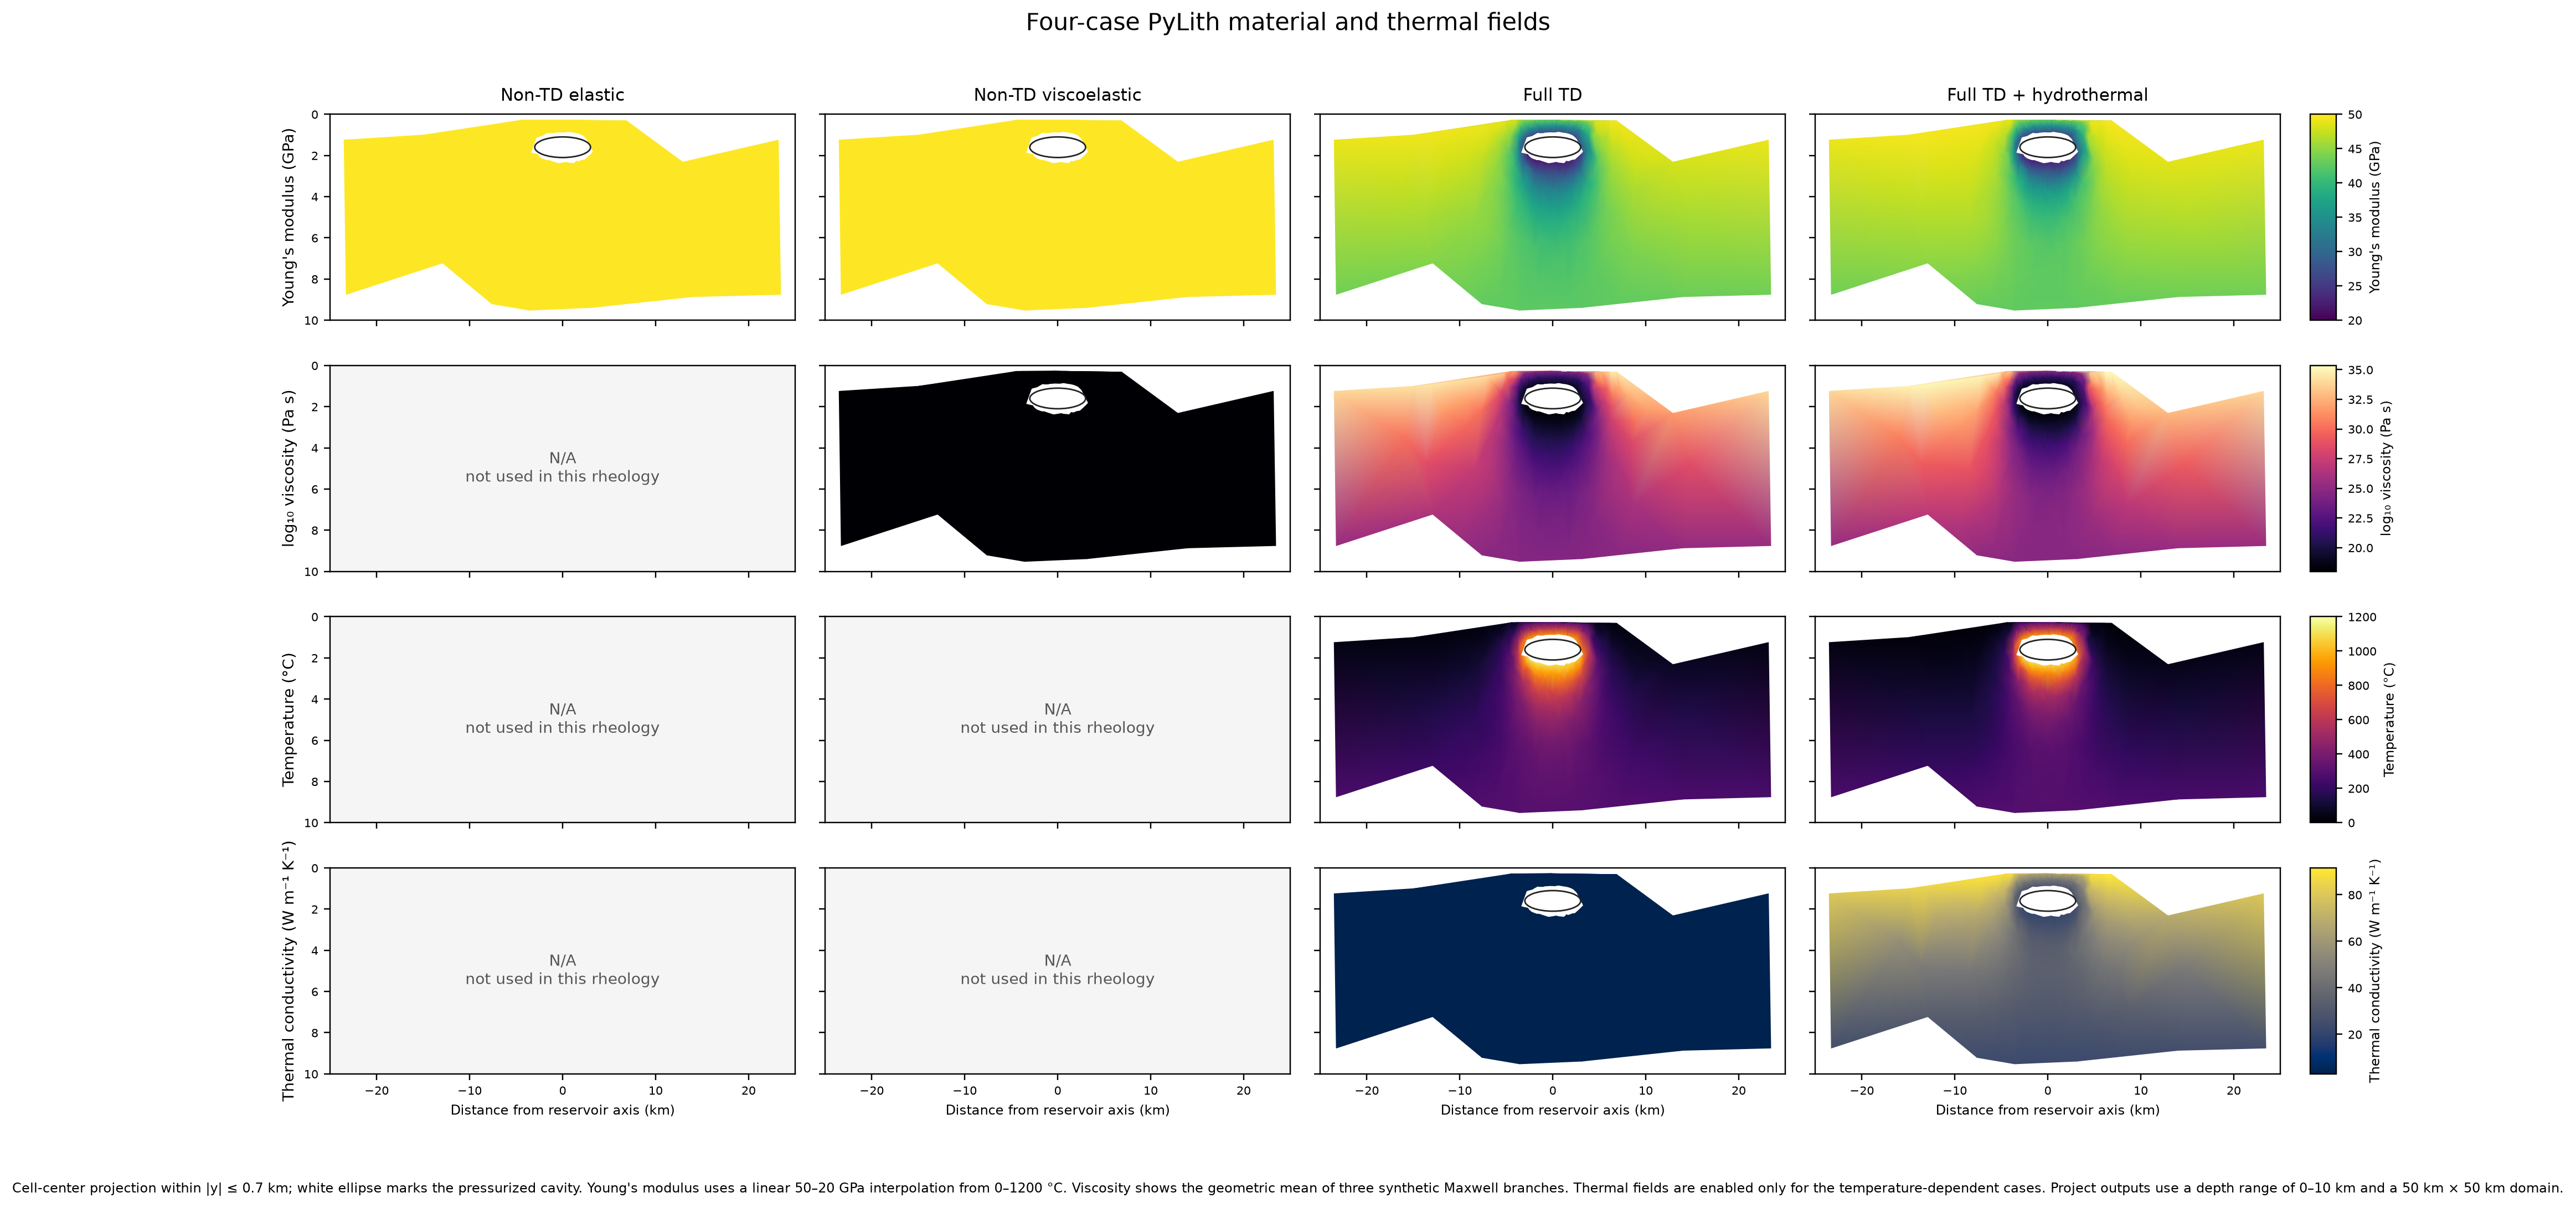
\includegraphics[width=\linewidth]{figures/figure3_rheology_property_matrix.png}
\tightcaption{Four project property cases under a shared synthetic load. The temperature-dependent and hydrothermal fields demonstrate that the property handoff runs; synthetic Maxwell branches, assumed boundaries, and the directed modulus law prevent interpreting this as a recovered paper result.}
\end{figure}

\begin{figure}[H]
\centering
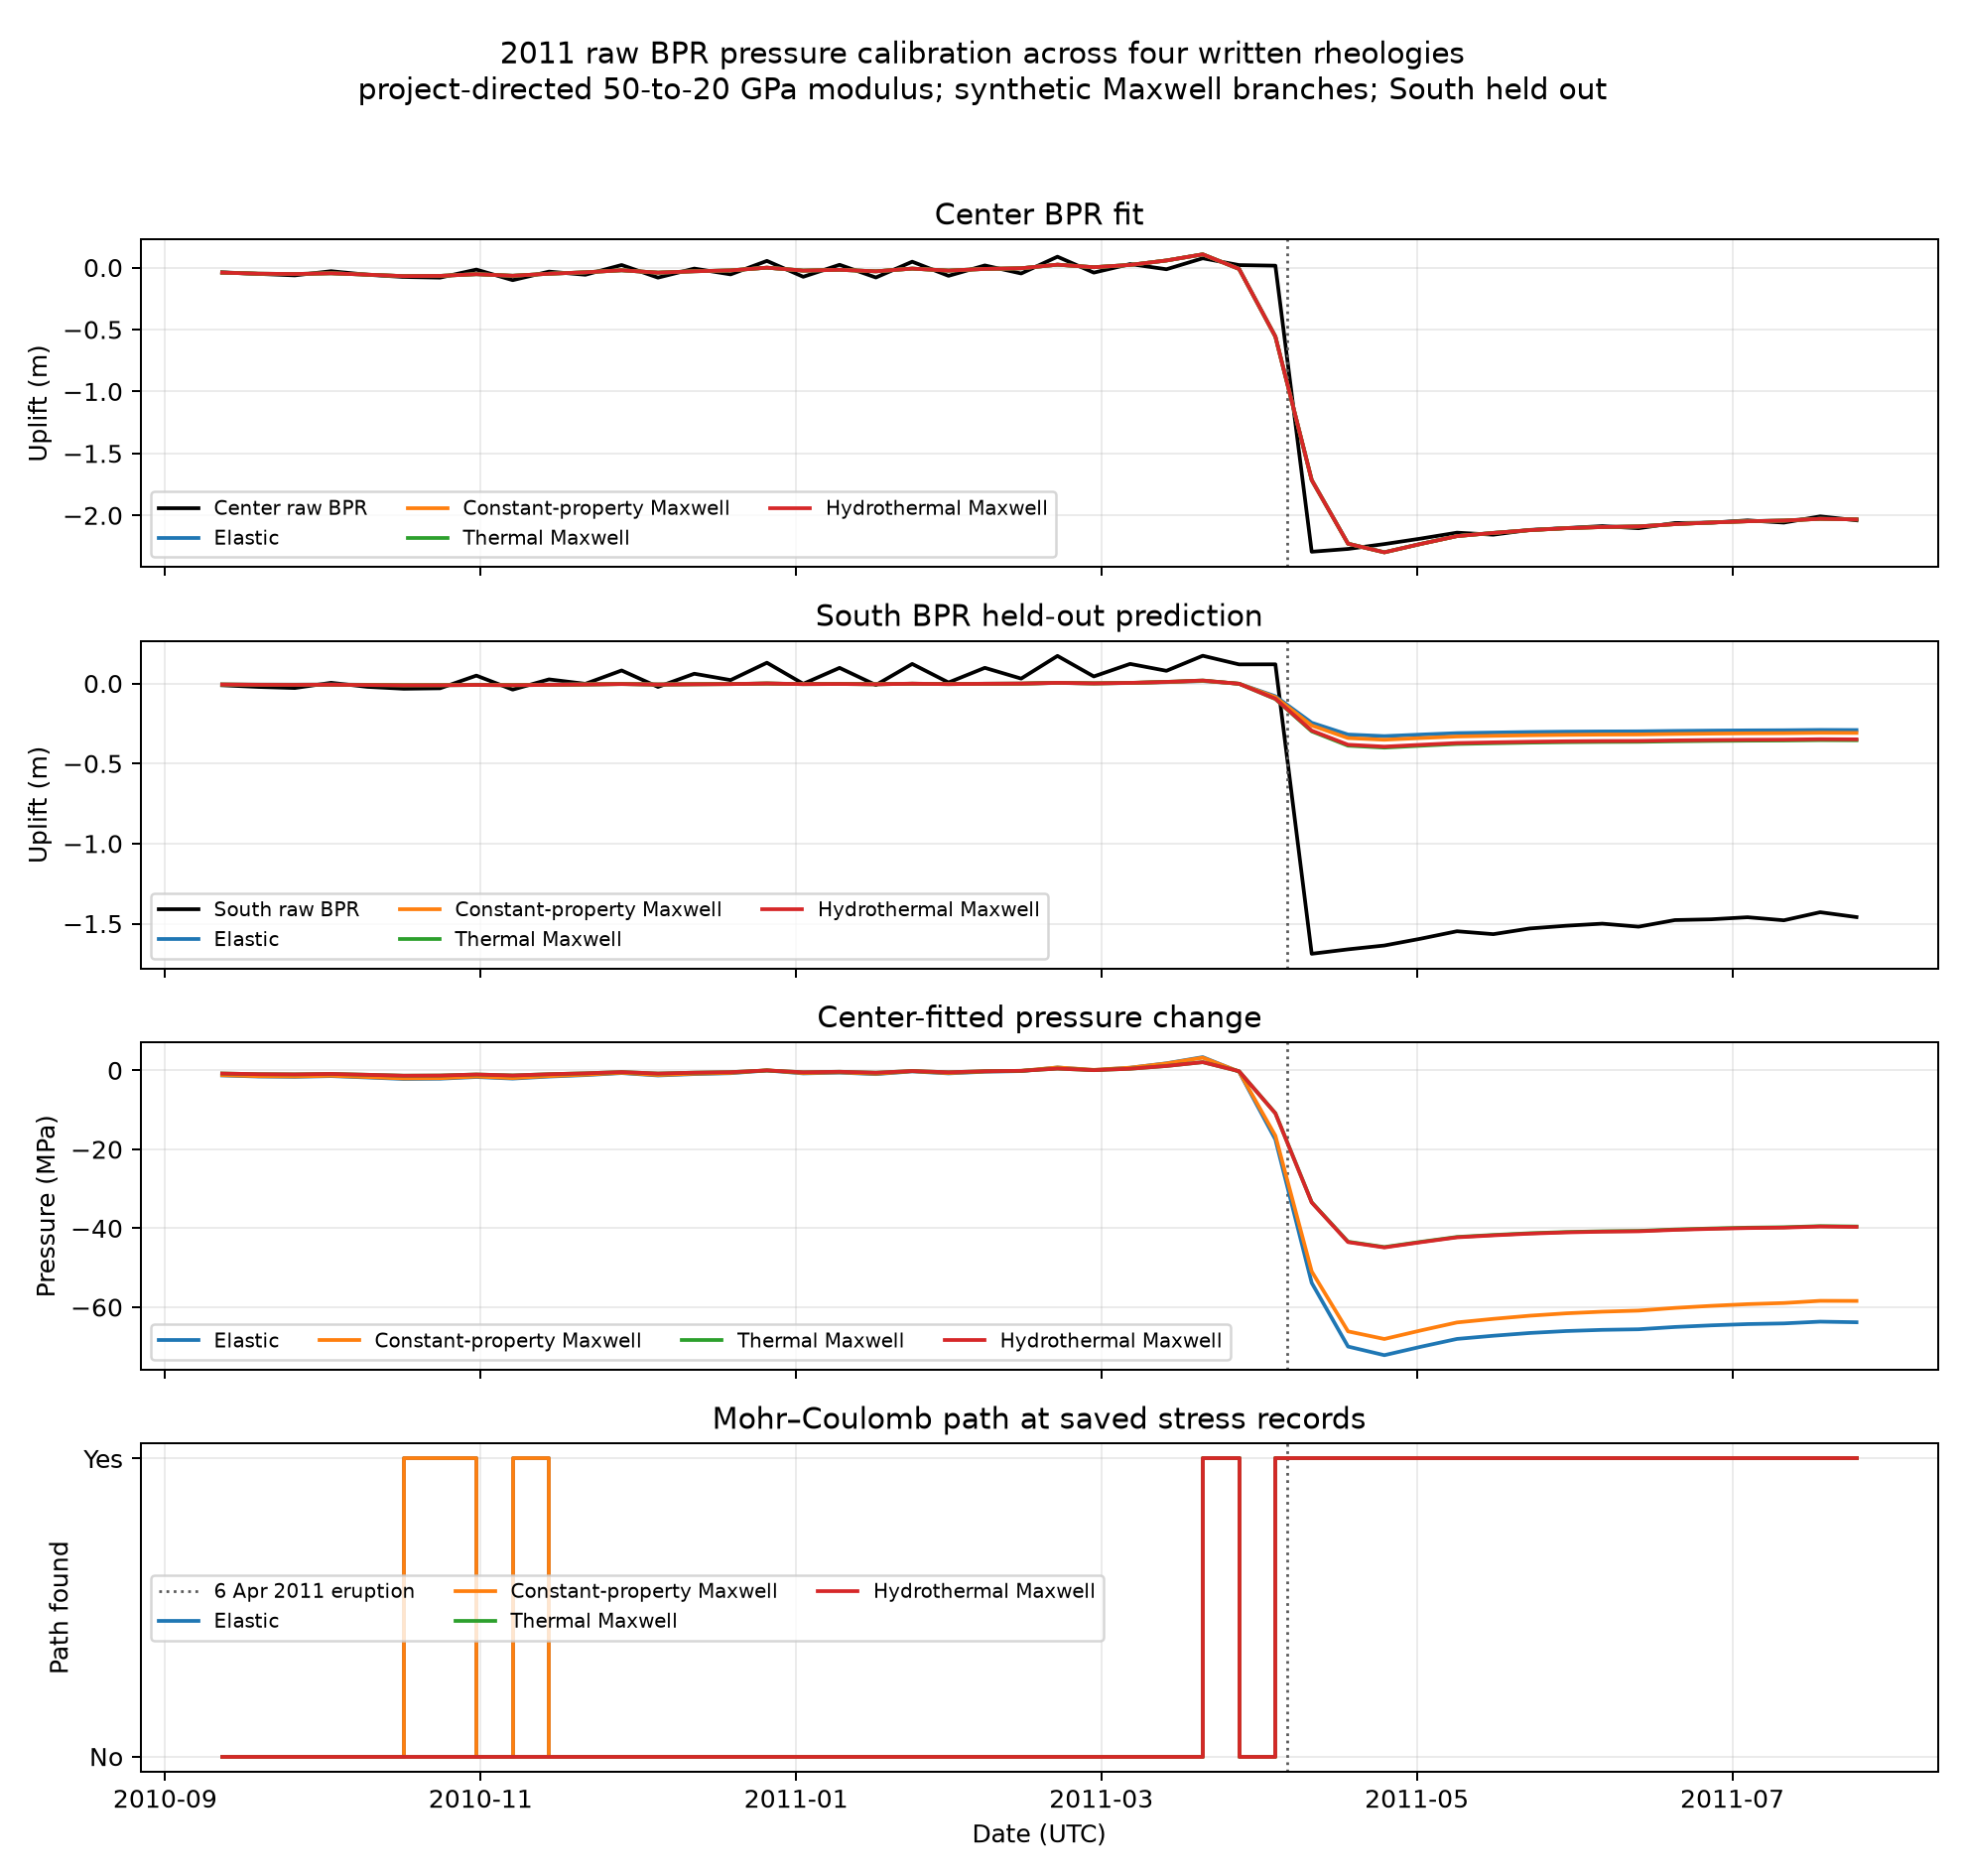
\includegraphics[width=\linewidth]{figures/historical_four_case_bpr_calibration.png}
\tightcaption{Current uncommitted 2011 raw-channel calibration. Center fit is close, while held-out South misses much of the observed deflation; the fit is retrospective and the inferred pressure is not measured.}
\end{figure}

\begin{figure}[H]
\centering
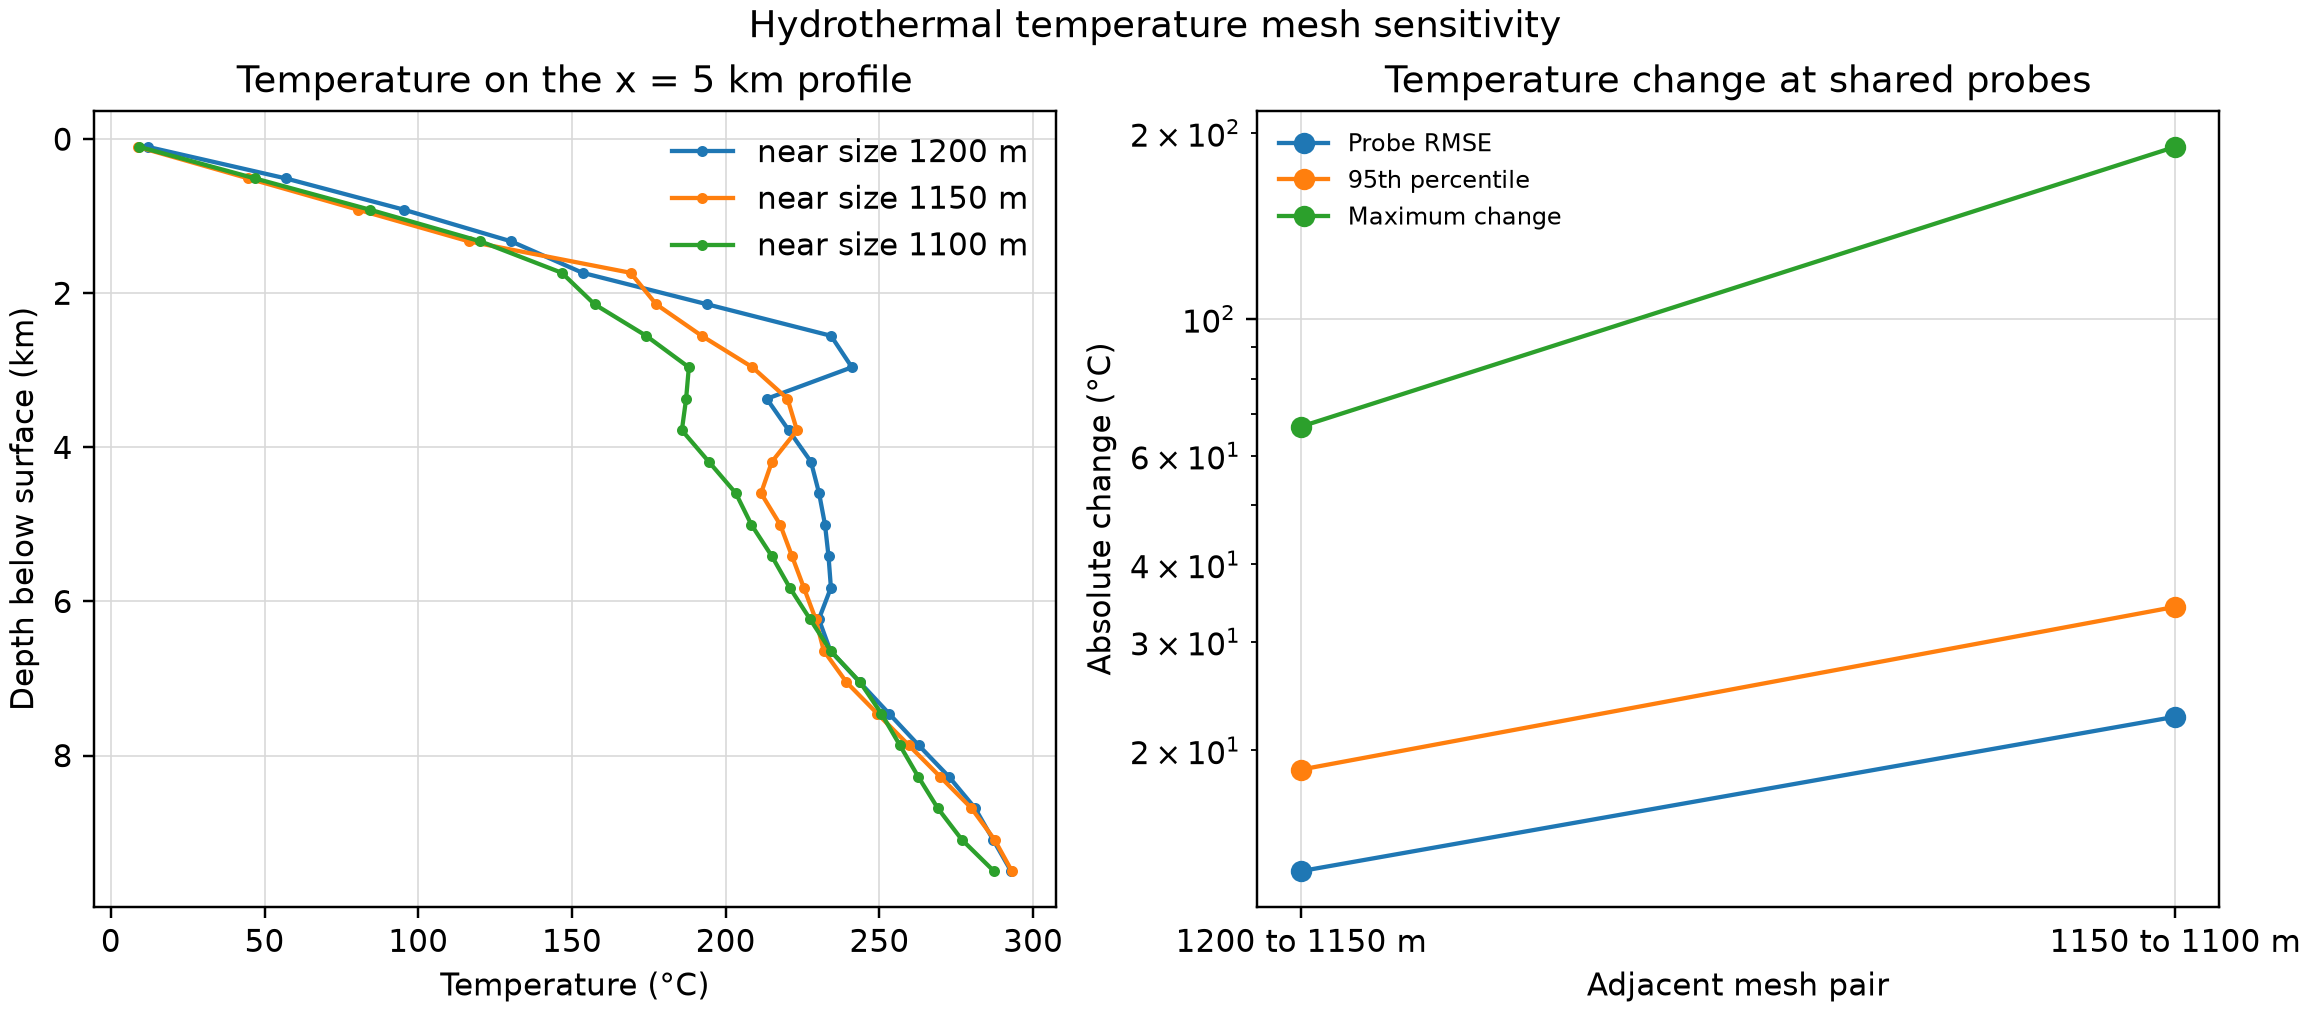
\includegraphics[width=\linewidth]{figures/thermal_mesh_sensitivity.png}
\tightcaption{Hydrothermal temperature probes on three independently generated meshes. Adjacent-pair probe RMSE is 12.8 and 22.7 $^\circ$C; maximum changes are 66.9 and 189.7 $^\circ$C. These are finite-probe differences, not a fieldwise convergence norm.}
\end{figure}

\begin{samepage}
\section*{Main obstacles, ranked}
\begin{enumerate}
\item \textbf{Numerical compliance and sampling (conclusion-changing).} Nonnested meshes, large response changes, and station samples still 50--500 m from surface vertices make pressure scale and spatial residuals provisional. The Mogi mismatch does not meet a documented agreement criterion.
\item \textbf{Missing or ambiguous physics (conclusion-changing).} The source leaves Poisson ratio, full-depth density, tensile strength, viscosity spectrum, friction conversion, and some loading details unresolved. The project chooses priors but cannot validate them. Hydrothermal cooling is a conductivity parameterization, not resolved circulation.
\item \textbf{Model departures and duration.} Main fits omit Winkler feedback and use a fixed base; the 22-year history is assembled from separated station deployments, and model forcing is limited to event windows or selected overlaps. No 2015 cycle hindcast, sustained failure test, permeability, or fault-slip model exists.
\item \textbf{Panel work.} Figure 1 is an independent geology map; the property matrix and selected pressure diagnostics are project-generated. Most failure and volume panels lack project fields or plots. Generating more panels before the first three issues are resolved would add little scientific evidence.
\end{enumerate}
\end{samepage}

The publisher-served supplement PDF in the worktree carries a ``Confidential manuscript submitted'' footer and may be a prepublication version. No local evidence indicates use of author code or numerical outputs. Raw observations and most simulation archives are ignored by Git, so the evidence trail is not portable from the public repository alone. The current calibration PNGs and JSON summaries also disagree with the checked-in figure inventory: this assessment reports the local JSON values and flags that mismatch below.

\clearpage
\onecolumn
\section*{Value of one bounded next step}
The estimates below are planning ranges, not charges. No per-agent usage records or provider pricing were present, so dollar equivalents cannot be verified. Use no more than one agent and no more than 20,000 agent tokens for the recommended gate; cap PyLith work at three unit-load runs and five minutes total wall time. Do not proceed to pressure recalibration or a larger mesh program until this gate and a human geomechanics review pass.

\small
\begin{tabularx}{\textwidth}{@{}p{0.18\textwidth}X p{0.2\textwidth}p{0.15\textwidth}p{0.16\textwidth}@{}}
\toprule
Question and work & Deliverable and success criterion & Main risk & Agent estimate & Compute estimate \\
\midrule
\textbf{Recommended: does mesh refinement stabilize station compliance?} Reuse the corrected N30$^\circ$W geometry; make three locally refined, nested or demonstrably comparable meshes; sample at exact BPR coordinates; run identical 1 MPa elastic unit loads. & A short compliance-versus-mesh report and figure. Pass only if the last two levels differ by $<5\%$ at both stations and exact-point sampling is resolved; otherwise stop pressure-calibration spending. & Gmsh may not produce nested meshes within the element cap; geometric and boundary errors may remain even if compliance stabilizes. & 12,000--20,000 tokens; range based on a bounded coding and evidence task. & Three single-core solves; target $<5$ min total under the repository's per-process limit. \\
\textbf{Human specification gate: which physical inputs are defensible?} Review density/prestress, modulus law, Maxwell spectrum, friction convention, tensile strength, and allowed pressure history against written sources and Axial measurements. & Signed input table that separates known values from priors and unresolved choices. Success requires an independent scientist to approve values or identify unavailable measurements. & Agent research cannot create missing observations or decide constitutive physics; the supplement may be prepublication. & 5,000--10,000 tokens for source indexing; scientific decision is human work. & No simulation; allow 1--2 hours of expert review. \\
\bottomrule
\end{tabularx}

\vspace{0.5em}
\textbf{Spending recommendation.} Approve only the first gate, with a 20,000-token agent ceiling and the five-minute compute cap, after a human confirms that exact station sampling is the relevant uncertainty. Stop if mesh comparability cannot be achieved within three runs, if either final compliance change exceeds 5\%, or if the gate passes but no defensible physical inputs are available. The token cap cannot be translated to dollars without the account's pricing and usage records; do not authorize an unpriced open-ended task.

\clearpage
\begin{landscape}
\section*{Appendix: panel inventory and evidence trail}
\scriptsize
Inventory count: 45 main-manuscript panels (including all 16 Fig. 3 property cells, 20 Fig. 5 slices, and four Fig. 6 concepts) plus six supplementary figure topics, 51 units total. Supplementary captions do not specify subpanel letters; supplementary figure pages were not inspected, so undocumented subpanels are not counted. ``Agreement'' means project checks only: no numerical comparison with publication model outputs, figure values, failure fields, or eruption predictions was used.

\vspace{0.4em}
\noindent
\begin{minipage}[t]{0.495\linewidth}
\begin{tabularx}{\linewidth}{@{}p{0.50in}p{0.82in}X@{}}
\toprule
Panel & Quantity & Data/plot paths; status, agreement, limitation \\
\midrule
1a & Bathymetry, flows, seismicity, reservoir proxies & \p{data/raw/figure1/}; \p{figures/figure1_axial_geologic_map.png}. Partial: independent sources; projection residual $<0.2$ m. Velocity contours are proxies, not official outlines; regional grid is not 1 m AUV bathymetry. \\
1b & Geometry and boundaries & \p{scripts/plot_model_setup_schematic.py}; \p{figures/model_setup_schematic.png}. Project schematic only. Fixed base remains in calibrations; thermal and spreading boundary details are assumed or unresolved. \\
2 & BPR deformation and earthquake counts & \p{data/processed/axial_historical_bpr/}; \p{figures/historical_bpr_deployment_context.png}, \p{figures/ooi_bpr_relative_uplift.png}. Partial independent observations, 1987--2026; no continuous history or earthquake-count series; no model comparison. \\
3 (16 cells) & Four properties by four rheologies & \p{data/processed/rheology_case_matrix_model_data.npz}; \p{figures/figure3_rheology_property_matrix.png}. Partial property handoff; stress reconstruction $\sim2\times10^{-16}$ relative $L_2$. Maxwell branches are synthetic; modulus map is project-directed. \\
4a & Reservoir pressure history & \p{data/processed/historical_four_case_bpr_calibration_1998/summary.json}; \p{data/processed/historical_four_case_bpr_calibration/summary.json}; \p{figures/historical_four_case_bpr_calibration_1998.png}, \p{figures/historical_four_case_bpr_calibration.png}. Partial, retrospective fits. Current raw South RMSE: 0.523--0.541 m (1998), 0.667--0.687 m (2011); pressure is inferred, not observed. \\
4b & Reservoir volume and deformation cycle & No volume-history archive or project plot located. Not implemented; source pressure/flux history and independent 2015 cycle calculation are absent. \\
5a--t (20) & Tensile and Mohr--Coulomb failure slices & Saved stress/failure tables under \p{data/processed/axial_historical_bpr/}; no corresponding 20-slice plot. Not implemented as panels. Failure-path outcomes depend on assumed strength, friction, mesh, and stress history. \\
6a--d (4) & Conceptual mechanism & No project data or plot. Not reproduced; no paper artwork copied. Any future concept should be a project schematic, not a traced panel. \\
\bottomrule
\end{tabularx}
\end{minipage}\hfill
\begin{minipage}[t]{0.495\linewidth}
\begin{tabularx}{\linewidth}{@{}p{0.50in}p{0.82in}X@{}}
\toprule
Panel & Quantity & Data/plot paths; status, agreement, limitation \\
\midrule
S1 & Modulus, viscosity, temperature, conductivity & \p{pylith/step12_generalized_maxwell_ellipsoid/output/hydrothermal-temperature.npz}; \p{figures/thermal_property_slices.png}; Fig. 3 matrix. Partial: one hydrothermal-section plot and a separate property matrix, not the full supplementary slice set. Eq. 16 conflicts with stated limits. \\
S2 & Brittle--ductile transition & Thermal archive above; no transition calculation or plot. Not implemented; transition criterion is not fully specified. \\
S3 & Mogi, viscoelastic/FEM, foundation benchmark & \p{pylith/step02_mogi_benchmark/output/}; \p{figures/ooi_mogi_calibration.png}. Not implemented as a panel: independent Mogi check has 44.9\% field error; Del Negro and prior FEM comparisons absent; no convergence. \\
S4 & Spring stiffness response & \p{data/processed/winkler_foundation_check.json}; \p{figures/winkler_foundation_check.png}. Not implemented as the requested sweep: one finite-spring/fixed-base diagnostic only; coarse-mesh station response is unstable. \\
S5 & Thermal and mechanical setup & \p{figures/model_setup_schematic.png}. Schematic only; numerical thermal field is not shown, and the target Winkler boundary is absent from main calibration. \\
S6 & Pressure by geometry and rheology & \p{data/processed/ellipsoid_mesh_sensitivity.json}; \p{figures/ooi_ellipsoid_elastic_calibration.png}. Not implemented: no converged compliance, multiple calibrated geometries, or pre-2014 pressure history. \\
\bottomrule
\end{tabularx}
\end{minipage}

\vspace{0.7em}
\textbf{Repository and provenance record.} HEAD is \texttt{e7d9dcc60d7c23203677f54a23abb9c3eba422fd}, equal to local \texttt{main} and \texttt{origin/main} at inspection. Worktree changes predated this assessment: \p{docs/figure_reproduction.md}; the two raw calibration PNG/PDF pairs; and \p{report/axial_model_report.tex} / \p{report/axial_model_report.pdf}. Untracked source PDFs are \p{cabaniss_et_al.pdf} and \p{cabaniss_supplement.pdf}. The raw calibration images changed materially from HEAD (60,739 and 266,930 differing pixels); their ignored current summaries are newer than the checked-in inventory, which records different South RMSE ranges. This report uses those local summaries and flags the mismatch; it does not overwrite the earlier report. No agent logs, token-usage records, or pricing data were found. Numerical summaries, raw archives, meshes, and HDF5 simulations are ignored by Git and will not be available from the public repository unless separately archived. The supplement is a publisher-served submitted-manuscript copy with a confidential footer. No evidence of prohibited author code, model output, plotting script, source data, or digitized figure values was found in the inspected records; the earlier agent history is unavailable, so provenance cannot be audited beyond the files and manifests present here.

\vspace{0.4em}
Supporting records: \p{docs/figure_reproduction.md}, \p{docs/paper_summary.md}, \p{docs/model_specification.md}, \p{docs/KNOWN_ISSUES.md}, \p{docs/run_log.md}, the local JSON summaries named above, and the saved solver logs under \p{pylith/step00_elastic_cavity/output/}, \p{pylith/step12_generalized_maxwell_ellipsoid/output/}, and \p{pylith/step16_winkler_foundation/output/}. The last recorded full reproduction at revision \texttt{3adb678} took 1,952 s and reports 120 passing tests and Ruff success; it predates HEAD. No full regeneration or new model run was performed for this assessment.
\end{landscape}
\end{document}
